
\subsection{Mechanistic Interpretation}

The reversal has a consistent physical description (Table~\ref{tab:mechanism}). SP's route
is about 8\,\% shorter than DTT's and that advantage is essentially constant across
regimes; what changes is the cost of using the shorter corridor. Between the lowest and
highest demand, implied in-network mean speed falls from 37.80 to 18.31\,km/h for SP, a
loss of 51.6\,\%, against 38.43 to 23.80\,km/h for DTT, a loss of 38.1\,\%, while emission
intensity rises from 255.1 to 590.7\,g/km for SP but only from 248.5 to 423.2\,g/km for
DTT. A fixed structural advantage is overtaken by a growing congestion penalty: at
720\,veh/h the policies achieve almost identical speeds and queueing, so DTT's longer route
is not compensated, whereas as demand rises the shortest corridor degrades faster than the
alternatives and the margin flips sign. Under arterial priority that corridor receives a
larger green share, consistent with the later crossing in Table~\ref{tab:margin}.

\begin{table}[htb]
\centering\small
\caption{Mechanism decomposition: SP minus DTT, averaged over the eight contexts at each
demand level. A negative distance difference means SP's route is shorter; a positive time
difference means SP is slower.}
\label{tab:mechanism}
\begin{tabular}{@{}lrrrrrr@{}}
\toprule
Demand & $\Delta$distance & $\Delta$in-network & $\Delta$insertion & $\Delta$journey
& $\Delta$\CO & $\Delta$stopped\\
& (m) & time (s) & delay (s) & time (s) & (g/veh) & (veh-s/veh)\\
\midrule
720\,veh/h & $-250.3$ & $-17.9$ & $0.0$ & $-17.9$ & $-44.7$ & $+6.4$\\
1200\,veh/h & $-288.0$ & $+84.8$ & $+18.1$ & $+102.8$ & $+322.5$ & $+104.1$\\
1680\,veh/h & $-277.2$ & $+113.7$ & $+441.2$ & $+554.9$ & $+416.9$ & $+114.3$\\
\bottomrule
\end{tabular}
\end{table}

This is a decomposition, not a causal identification. The experiment varies demand and
green split but does not isolate movement-level mechanisms, and the per-run aggregates
contain no per-approach delay, stop count or route-share breakdown.

\subsection{Context-Aware Selection}
\label{sec:selection}

\begin{figure}[tb]
\centering
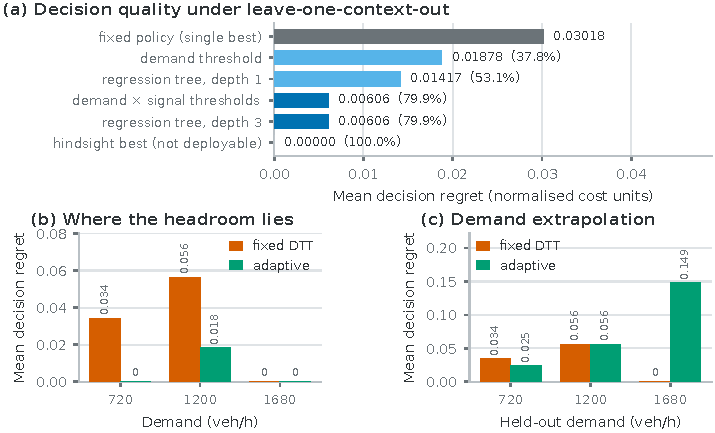
\includegraphics[width=\linewidth]{figures/fig4_decision.pdf}
\caption{(a) Mean decision regret of every rule in the ladder under
leave-one-context-out, with the percentage of headroom captured. (b) Where the headroom
lies: at 1680\,veh/h the fixed policy is already optimal. (c) Leave-one-demand-out. When
the withheld demand level lies above the fitted support the adaptive rule is
substantially worse than the fixed policy it replaces.}
\label{fig:decision}
\end{figure}

\begin{table}[htb]
\centering\small
\caption{Selection rules under leave-one-context-out. Everything --- reference scales,
thresholds, tree and the identity of the best fixed policy --- is refitted inside each
fold. Mean and max are decision regret in normalised cost units; ``lowest cost'' counts
contexts in which the chosen policy is the observed best; ``captured'' is $G(\pi)$ of
Eq.~\eqref{eq:headroom}.}
\label{tab:ladder}
\begin{tabular}{@{}llrrcr@{}}
\toprule
& Rule & Mean & Max & Lowest cost & Captured\\
\midrule
R0 & Single best fixed policy & 0.03018 & 0.13176 & 10/24 & ---\\
R1 & Demand threshold & 0.01878 & 0.13176 & 18/24 & 37.8\,\%\\
R3 & Regression tree, depth 1 & 0.01417 & 0.10079 & 17/24 & 53.1\,\%\\
R2 & Demand $\times$ signal thresholds & 0.00606 & 0.11545 & 21/24 & 79.9\,\%\\
R4 & Regression tree, depth 3 & 0.00606 & 0.11545 & 21/24 & 79.9\,\%\\
R5 & Hindsight best (not deployable) & 0.00000 & 0.00000 & 24/24 & 100\,\%\\
\bottomrule
\end{tabular}
\end{table}

Table~\ref{tab:ladder} and Fig.~\ref{fig:decision}a report the ladder under the identical
held-out protocol. The central result is the equality of rows R2 and R4: a rule with two
free parameters, one demand threshold per signal plan, reproduces the regression tree
exactly --- same mean regret, same maximum regret, the same 21 contexts chosen correctly.
The fitted models explain why: in all 24 folds the tree splits first on demand at
1440\,veh/h, then on signal plan, then on demand again at 960\,veh/h, while the explicit
rule fits thresholds of 960\,veh/h under balanced timing and 1440\,veh/h under arterial
priority in every fold. The two rules are the same rule.

This bounds what the learned model contributes: the 79.9\,\% is produced by the regime
structure of Section~6.2, not by model capacity, and a practitioner would obtain the same
decisions from two numbers written on a page. Feature ablation agrees --- removing the
restriction configuration leaves the result unchanged at 79.9\,\%, whereas removing the
signal plan reduces it to 72.9\,\%. The ladder also separates prediction quality from
decision quality: the depth-3 model predicts poorly in absolute terms, with held-out mean
absolute error of 44.6\,s in journey time and 82.4\,g in \CO\ against benchmark means of
542.8\,s and 1263.5\,g, yet chooses the lowest-cost policy in 21 of 24 contexts, because
errors that preserve the ordering of three policies cost nothing. This is the
predict-then-optimise distinction of~\cite{elmachtoub2022smart} in a traffic setting, and
it means reporting the selector's regression accuracy would misdescribe its usefulness.

\paragraph{The extrapolation boundary.}
The leave-one-demand-out experiment reverses the conclusion (Fig.~\ref{fig:decision}c).
Pooled over the three folds, mean regret rises to 0.07649, above the 0.03018 of the fixed
policy: applied this way the procedure is worse than doing nothing adaptive. The folds are
not equivalent. With 1200\,veh/h withheld the test point lies between two training levels
and the selector reproduces the fixed-policy regret of 0.05633 exactly, gaining nothing;
with 720\,veh/h withheld it never sees a context in which SP is optimal and incurs 0.02456
against 0.03422, slightly better only because the fixed policy is also wrong there; and
with 1680\,veh/h withheld the test point lies above the training range, DTT is optimal in
all eight withheld contexts, the selector assigns TECO10 to half of them, and it incurs
0.14856 where the fixed policy incurs zero.

The failure is specific and diagnosable rather than general: a tree cannot extrapolate,
returning beyond the largest training value of a feature the prediction of its outermost
leaf, which here was fitted where TECO10 was competitive. Interpolation inside a
represented range is safe in this benchmark, extrapolation beyond it is not, and a model
that produces a prediction outside its support is not thereby producing a usable one.

\subsection{Multi-Criteria and Pareto Structure}
\label{sec:multicriteria}

\begin{figure}[tb]
\centering
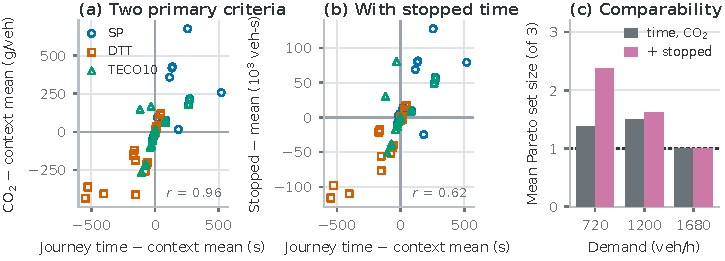
\includegraphics[width=\linewidth]{figures/fig5_pareto.pdf}
\caption{Multi-criteria structure. (a, b) Policy outcomes expressed as deviations from
their own context mean, which isolates the comparison that decides a context; $r$ is the
mean within-context correlation across the three policies. (c) Mean number of
non-dominated policies per context, with and without the congestion axis.}
\label{fig:pareto}
\end{figure}

Whether a preference model does any work depends on how independent the criteria are.
Within a context --- the comparison that determines which policy wins --- the mean
correlation between mean journey time and \CO\ across the three policies is 0.96
(Fig.~\ref{fig:pareto}a), so the two primary criteria are close to collinear, which is why
the weight sweep below changes nothing; the corresponding correlation between journey time
and network stopped vehicle-time is 0.62 (Fig.~\ref{fig:pareto}b), so the congestion
diagnostic carries information the primary criteria do not.

Treating that diagnostic as a third axis changes comparability but not the decision. Under
the two primary criteria the mean Pareto set contains 1.29 of the three policies and 17 of
24 contexts have a single non-dominated policy; adding stopped vehicle-time raises the
mean set to 1.67 and leaves only 12 such contexts, the effect concentrated at low demand
where the mean set size rises from 1.38 to 2.38. At 1680\,veh/h it remains 1.00 under
both, DTT dominating outright on all three axes. Crucially, the policy chosen by the
primary rule is non-dominated in the three-criterion sense in all 24 contexts, so the
reported decisions are never Pareto-dominated once congestion is included. An equal-weight
additive rule over all three criteria agrees with the primary rule in 22 of 24 contexts
--- the exceptions being the balanced central-restriction context at 720\,veh/h and the
balanced upper-restriction context at 1200\,veh/h --- and ranking by stopped vehicle-time
alone agrees in 18 of 24. The congestion diagnostic therefore reduces the \emph{confidence}
with which policies can be ordered at low demand, where they differ little on any axis,
without altering the regime structure or the decisions. That is also why it was not
promoted to a primary criterion: it would have changed the meaning of the reported
decisions while changing almost none of them.

\subsection{Robustness and Negative Controls}
\label{sec:robust}

\begin{table}[htb]
\centering\small
\caption{Sensitivity checks under the primary protocol. ``Captured'' is the fraction of
headroom recovered; ``labels changed'' counts contexts in which the preferred policy
differs from the primary analysis. All 15 depth/leaf settings capture positive headroom.
The two negative controls are described in the text. $^{\ast}$On the in-network scale the
headroom is 0.03305 rather than 0.03018.}
\label{tab:robust}
\setlength{\tabcolsep}{4pt}
\begin{tabular}{@{}lll@{}}
\toprule
Variation & Captured & Labels changed\\
\midrule
Primary analysis (depth 3, leaf 2, $w=0.5$) & 79.9\,\% & ---\\
Depth $\in\{1,2,3,4,\infty\}\times$ leaf $\in\{1,2,3\}$ & 50.9--79.9\,\% & --- \\
Weight $w_{\text{time}}$ swept $0\rightarrow1$ & 78.1--81.7\,\% & 0 of 24 decisions\\
Seed-block hold-out, three blocks & 60.8, 67.7, 90.2\,\% & ---\\
Training-only scoring scales & 79.8\,\% & ---\\
In-network time replaces journey time & 80.1\,\%$^{\ast}$ & 0 of 24\\
95th percentile replaces the mean & --- & 2 of 24\\
Route distance as a third criterion & --- & 0 of 24\\
Stopped vehicle-time as a third criterion & --- & 2 of 24\\
\bottomrule
\end{tabular}
\end{table}

Table~\ref{tab:robust} collects the checks of Section~5.4; the held-out advantage survives
all of them. Both negative controls fire, and both constrain the paper's own claims.

The emission-forecast control is the reason ECO is not in the decision portfolio. Its
aggregate accuracy is acceptable --- selected-path emission WAPE of 14.71\,\% against a
25\,\% criterion and signed bias $-0.32$\,\% against a 10\,\% criterion --- yet in a
fixed-replay probe over all 29 admissible routes it identified the best route in only 3 of
8 panels, with a mean relative selection loss of 21.62\,\% and a worst case of 78.16\,\%.
Good average forecast accuracy did not produce good route choices, the
accuracy--decision gap of Section~\ref{sec:selection} in the opposite direction. ECO is
also outcome-identical to SP in 21 of 24 contexts here. Neither observation is evidence
that eco-routing is ineffective in general; both are statements about this estimator in
this environment.

The preference-model control is a negative result about this study's own apparatus:
sweeping the time weight from 0 to 1 leaves every selector decision unchanged and changes
the hindsight winner in a single context, so the multi-criteria layer is doing almost no
work here. Adding further multi-criteria methods would produce agreement among methods
rather than evidence about the traffic system, and we therefore report the additive model
as a transparent definition of ``preferred'' rather than as a contribution.

\subsection{Implications and Limitations}

The three questions of Section~1 receive different answers, and the differences are the
point: the preferred policy changes with regime, the decision value of that change is real
but small and localised, and the recovery is deployable only inside the represented
regimes. For practice this suggests a modest design --- commit first to the right fixed
policy, which is where most of the available cost sits, then add adaptation as two demand
thresholds conditioned on the active signal plan, with a declared operating domain
monitored against the demand range used to fit it and a fixed-policy fallback outside it.

The limitations are concrete. \emph{External validity:} one synthetic topology, one primary
origin--destination structure, specified rather than calibrated lane capacities and a
homogeneous fleet, so the brackets, headroom and capture percentages are benchmark-specific
quantities. \emph{Resolution:} 24 contexts, three replications and a demand grid of
480\,veh/h; the experiment brackets the preference change rather than locating it, the runs
that would locate it were not available (Section~\ref{sec:boundary-exp}), two of the 24
margins are unresolved, and leave-one-context-out estimates procedure quality on folds that
share most of their training contexts. \emph{Behaviour:} restrictions are announced,
compliance is complete and routes are assigned once at departure, so nothing here speaks to
heterogeneous compliance, en-route control, or the feedback that would arise if a large
share of traffic followed the same guidance. \emph{Criteria and measurement:} the two
primary criteria are nearly collinear here, so the preference model is close to inert;
journey time includes insertion delay while in-network \CO\ does not, which leaves the
ordering unaffected but not the absolute values at the highest demand; and the congestion
diagnostic is measured over all vehicles rather than the cohort. \emph{Mechanism:} the
per-run aggregates support a consistent decomposition of the reversal but not a causal
attribution to particular movements or signal phases. \emph{Scope:} the review is targeted
rather than systematic, and the paper accordingly claims no priority.

\section{Conclusion}

This study treats the choice of a routing policy as a context-dependent decision problem
and evaluates it on a controlled signalised benchmark of 432 completed SUMO runs over 24
contexts. Shortest-distance routing has the lowest observed cost in all eight low-demand
contexts and dynamic travel-time routing in all eight high-demand contexts, with the
crossing displaced by at least one demand step under arterial-priority timing, and all
three portfolio policies win somewhere, so the portfolio is complementary.

Complementarity, however, is not decision value. The single best fixed policy leaves only
0.03018 normalised cost units of headroom, of which a leave-one-context-out selector
recovers 79.9\,\% --- a share of attainable decision quality, not a physical improvement
rate; the corresponding physical differences are 13.00\,s and 30.71\,g per vehicle, while
choosing the worst rather than the best fixed policy costs 0.28807 units. A two-threshold
rule on demand and signal plan matches the fitted regression tree exactly, so the
recoverable value comes from the regime structure and not from model capacity.

Decision value is in turn not deployability. When an entire demand regime is withheld,
pooled regret rises to 0.07649, above the fixed-policy benchmark, and in the fold that
extrapolates above the training range the adaptive rule incurs 0.14856 where the fixed
policy incurs nothing. The recommendation is therefore conditional and operationally
specific: context-dependent routing-policy selection is worth deploying only within an
explicitly declared regime domain, implemented as a small number of interpretable
thresholds, with a fixed-policy fallback whenever the operating context leaves it.
Establishing where inside the observed brackets the preference actually changes requires
intermediate-demand simulations on this same network, which remain to be run.

\bibliographystyle{splncs04}
\bibliography{references}

\end{document}
